%% Ingenieur article: a dual-path voice interface for drone-swarm formation control
%% on a Raspberry Pi 5, with reflex preemption of a small language model.
%% Elsevier CAS double-column template (cas-dc, els-cas-templates 2024).
%% Build: pdflatex main -> bibtex main -> pdflatex main -> pdflatex main
%% (or upload this folder, including thumbnails/ and figures/, to Overleaf).

\documentclass[a4paper,fleqn]{cas-dc}

\usepackage[authoryear]{natbib}
%% Local builds without the STIX/Charis fonts fall back to Latin Modern (vector) instead of
%% bitmap Computer Modern; on Overleaf, where STIX is installed, this line does nothing.
\IfFileExists{stix.sty}{}{\usepackage{lmodern}}
\usepackage{xurl}
%% Long model names (e.g. Qwen2.5-0.5B-Instruct) cannot hyphenate; allow a little extra stretch.
\setlength{\emergencystretch}{2em}
\usepackage{tikz}
\usetikzlibrary{fit,backgrounds}

%% Change tracking for the step-2 peer review (articles/REVIEW_step2_peer_review.md); the IDs
%% (P1, P3, ...) are the rows of its prioritised action plan. Step-1 audit markup is accepted.
%% cas-dc already defines \comment, so the margin note of `changes' is \chcomment here.
\usepackage[draft,commandnameprefix=ifneeded]{changes}   % switch to [final] to strip all markup before submission
\definechangesauthor[name={Review}, color=blue]{PR}
\setaddedmarkup{{\color{blue}#1}}
\setdeletedmarkup{{\color{red}\sout{#1}}}
\setlength{\marginparwidth}{1.2cm}
\setuptodonotes{size=\tiny}
%% Inside floats, where margin notes cannot go, the finding ID is printed inline instead. Whole
%% blocks (a list) cannot be struck through, so they are coloured instead. Like the rest of the
%% markup, all of this disappears under [final].
\makeatletter
\newcommand{\AuditID}[1]{\ifbool{Changes@optiondraft}{\textsuperscript{\color{blue}\tiny[#1]}}{}}
\newcommand{\AuditDeletedBlock}[1]{\ifbool{Changes@optiondraft}{{\color{red}#1}}{}}
\newcommand{\AuditAddedBlock}[1]{\ifbool{Changes@optiondraft}{{\color{blue}#1}}{#1}}
%% A table row cannot sit inside a group, so a deleted row is dropped whole under [final] and
%% shown, cell by cell struck through, in draft.
\newcommand{\AuditDeletedRow}[1]{\ifbool{Changes@optiondraft}{#1}{}}
\makeatother

\newcommand{\QF}{Q4\_K\_M}

%% The template always prints an "ORCID(s):" footnote line. It is suppressed until the
%% authors' ORCID iDs are added (\author[1]{Name}[orcid=0000-0000-0000-0000]); then delete it.
\renewcommand{\printorcid}{}

\begin{document}
\let\WriteBookmarks\relax
\def\floatpagepagefraction{1}
\def\textpagefraction{.001}

\shorttitle{A dual-path voice interface for drone-swarm control on a Raspberry Pi 5}
\shortauthors{T. Kahia and B. Khaldi}

\title [mode = title]{A dual-path voice interface for drone-swarm formation control on a
Raspberry Pi 5: reflex preemption of a small language model}

\author[1]{Tayeb Kahia}
\cormark[1]
\ead{tayeb.kahia.ai@gmail.com}
\credit{Conceptualization, Methodology, Software, Investigation, Data curation, Formal analysis,
Visualization, Writing -- original draft}

\author[1]{Belkacem Khaldi}
\ead{<email-author-2>}   % PLACEHOLDER: Khaldi's e-mail
\credit{Conceptualization, Methodology, Supervision, Writing -- review \& editing}

\affiliation[1]{organization={\'Ecole Sup\'erieure en Informatique -- 08 Mai 1945},
            city={Sidi Bel Abb\`es},
            country={Algeria}}

\cortext[1]{Corresponding author.}

\begin{abstract}
A language-model voice interface is slow to stop a drone swarm: its parser cannot start before
the operator finishes speaking. Our interface runs its speech and language stages on a Raspberry
Pi~5 and splits commands between two paths. A parse path
transcribes each utterance and parses it with a fine-tuned small language model under a grammar; a
reflex path, a two-class keyword spotter, publishes a hold or an abort without transcription and
cancels any parse in progress. A two-test rule admits to the reflex path only commands whose delay
changes the outcome and whose false trigger can only make the swarm do less: two of ten. On recorded audio, each of 39 keyword takes that met a parse cancelled
it, with no class confusion.\added[id=PR]{ Through the parse path alone, the same takes waited 612~ms at the
median for the end of speech, and 3 of 40 stops became a formation command.}\AuditID{P12} Both paths miss their latency budgets: the reflex path takes 545--556~ms
at the 95th percentile against 150~ms, almost all of it before the board's 5--18~ms, and the parse
path 3,122~ms against 2,500~ms. Under rotor
noise, command recognition falls from 0.690 to 0.590 at 10~dB, and almost no failure resolves to
a hold. The rule
and the budget carry over to other voice interfaces, and the misses locate what to change next:
the spotter's decision delay, the recogniser and prompt caching. No physical flight or
live-microphone run was performed.\AuditID{rewritten: P18, P16}
\end{abstract}

\begin{highlights}
\item \replaced[id=PR]{Stop commands bypass the language model through a keyword-spotter reflex path}{A keyword-spotter reflex path preempts a small language model on a Raspberry Pi 5}\AuditID{P18}
\item \replaced[id=PR]{A two-test rule admits only hold and abort to the reflex path}{A two-test membership rule admits only hold and abort to the reflex path}
\item \replaced[id=PR]{Each of 39 keyword takes met during inference cancelled the decode}{All 78 reflex triggers during inference cancelled the decode in progress}\AuditID{P16}
\item \replaced[id=PR]{Reflex p95 is 545 ms against 150 ms; post-detection board time is 5--18 ms}{Reflex latency misses its budget before the board; the board adds only 6--18 ms}
\item Rotor noise lowers command recognition from 0.690 (clean) to 0.590 at 10 dB
\end{highlights}

\begin{keywords}
Voice control \sep Drone swarms \sep Keyword spotting \sep Edge inference \sep
Small language models \sep Formation control
\end{keywords}

\maketitle

% =============================================================================
\section{Introduction}
\label{sec:intro}

A voice interface lets one operator command a group of drones as a unit, with eyes on the airspace
rather than on a screen: an utterance such as ``form a circle with radius five metres'' addresses
five vehicles at once. Language models have made such interfaces flexible, turning free phrasing into
plans, programs or structured commands~\citep{saycan2022,chatgptrobotics2024,typefly2024}. Most of
these systems run the model on a server or a GPU. At an outdoor site without assured connectivity,
the interface has to run on the operator's own device, and on a small single-board computer every
stage of the speech chain costs on the order of a second.

That cost is acceptable for a formation change and not for a stop. A parser that transcribes and
interprets an utterance cannot start until an endpointer has decided that the operator has
finished speaking, and that wait alone is longer than a stop can afford\added[id=PR]{ (612~ms at the median after
the end of a recorded stop phrase, Section~\ref{sec:res-single})}\chcomment[id=PR]{P12}. Routing a stop through the
same path as every other command therefore delays it by the whole cost of interpretation. Routing it
through a faster path that does not interpret speech raises a different problem: a false trigger on
such a path publishes a well-formed command that no later check can distinguish from a spoken one.
Which commands may take such a path is therefore a safety question, and it is not answered by the
systems we reviewed.

This article presents a voice interface for a swarm of five drones whose speech and language stages all run on a
Raspberry Pi~5, with no cloud service, and addresses both problems. A companion paper selects and evaluates the language
model it uses~\citep{companion}; here we describe and evaluate the system built around it. \replaced[id=PR]{The contributions are:}{The contribution we claim is narrow:}
\AuditDeletedBlock{%

\begin{itemize}
\item A membership rule for a path that bypasses interpretation: a command qualifies only if its
  delay changes the physical outcome and its unprompted execution can only make the swarm do less.
  For the ten intents of the schema the rule admits exactly two, a hold and an abort, and it states
  the condition under which a third class could be admitted.
\item A latency budget of that path's own, specified per stage and measured on the board while
  the language model decodes on the same processor.
\end{itemize}
To measure them we built a dual-path runtime in which a keyword-spotter \emph{reflex path}
preempts language-model inference on the \emph{parse path}, with an ordering rule that prevents a
stale command from overriding a stop, and a three-layer validation chain. These are engineering,
not claimed as novel: preemption of a slower path by a fast gate is prior art~\citep{mira}, and
the decoding grammar is the companion paper's. We evaluate both paths against the budget, idle and
under load, together with keyword-spotter error rates, recognition under rotor noise including the
direction of the errors, and formation control of five simulated drones, and report every missed
target.}%
\AuditAddedBlock{%
\begin{itemize}
\item A membership rule for commands that bypass interpretation: a command qualifies only if its
  delay changes the physical outcome and its unprompted execution can only make the swarm do less.
  Applied to a ten-intent schema it admits exactly a hold and an abort, and it states the condition
  under which a third class could be admitted.
\item A per-stage latency budget for that path, measured on the board while the language model
  decodes on the same processor, which separates the spotter's decision delay (540~ms at p95) from
  the board's own share (5--18~ms).
\item An open, CPU-only implementation used to measure both: a dual-path runtime with preemption,
  an ordering rule that keeps a stale command from overriding a stop, and three validation layers,
  evaluated against every target, with each miss located.
\end{itemize}
Preemption of a slower path by a fast gate is prior art~\citep{mira}, and the decoding grammar is
the companion paper's; what this article adds is the rule that restricts the fast path and the
budget against which its latency is located.}\AuditID{P18}

Section~\ref{sec:related} reviews the closest work, Section~\ref{sec:methods} describes the system and
the experimental setup, Section~\ref{sec:results} reports the measurements,
Section~\ref{sec:discussion} discusses them, and Section~\ref{sec:conclusion} concludes.

% =============================================================================
\section{Related work}
\label{sec:related}

\paragraph{Voice and language interfaces for drones and swarms.} Early voice control confined the
operator to a fixed command language matched by regular expressions or by phonemes of a domain
vocabulary~\citep{landau2017,contreras2020}. Language models replaced the fixed language with
generated plans and programs, checked by a human on the loop~\citep{chatgptrobotics2024} or
grounded in a robot's skills~\citep{saycan2022}. Drone-specific agents make latency explicit:
TypeFly streams a compact plan language from a remote GPT-4 and keeps response time below
1.5~s~\citep{typefly2024}, and the agent of \citet{lim2025} prompts open models on a local
workstation GPU. \citet{silva2026} treat the model as an untrusted commander validated on a
server, \citet{sikorski2025} run recognition offline beside a local model on a GPU-equipped
computer, and \citet{torkamani2025} route between a model on a Jetson board and the cloud.\added[id=PR]{
\citet{nguyen2026fme} split the chain between a Raspberry Pi, for speech recognition, and a Jetson
Orin NX, for an 8~B model, and \citet{ahmed2026} run a fine-tuned small parser without a cloud
service.}\chcomment[id=PR]{P6} For swarms, SwarmChat offers voice and text
through rule-based intent matching~\citep{swarmchat2025}; \citet{iannoli2026} evaluate
general-purpose models on swarm missions in software-in-the-loop simulation; SkySim places a
cloud-hosted planner above a potential-field layer and holds position when a waypoint is
rejected~\citep{skysim2026}; and CommandSwarm gates generated behaviour trees with a deterministic
parser and a safety classifier~\citep{commandswarm2026}. We build on these ideas: deterministic
gating, hold on rejection and a separation layer below the planner are prior art. None of these
systems reports running its speech and language chain on a single-board computer without a GPU, and none
carries a stop outside the path that interprets commands under a latency budget of its own.

\paragraph{Fast-path and dual-path architectures.} Several systems pair a fast path with a slower
one. \citet{simoes2024} and \citet{henry2026} compare a direct speech-to-command classifier with a
recognition-plus-language-model cascade as alternatives; the fast path replaces the cascade rather
than accompanying it. \citet{dualattn2023} use wake-word detection to choose a cheaper branch inside one
recognition model. RelayS2S commits a fast spoken draft when a learned verifier accepts
it~\citep{relays2s}. MIRA is closest to our design: a gate on voice activity aborts a robot's
response and motion, preempting a slower deliberative path~\citep{mira}. Its fast path carries one
action and states no latency target, and none of these works states which commands a fast path may
carry.

\paragraph{Swarm formation and separation.} Formation controllers commonly combine slot
assignment~\citep{turpin2014} with artificial potential fields~\citep{khatib1986}, whose failure
modes are well documented~\citep{koren1991}, and with flocking terms~\citep{reynolds1987}.
\citet{llm2swarm2024} distinguish language models that synthesise controllers from models embedded
in each robot; like SkySim, our system uses a single model instance that issues formation-level
commands to a conventional controller.

\paragraph{Gap.} No reviewed system specifies which commands may bypass interpretation, or a
latency budget for a stop measured while a language model decodes on the same processor. We address
both, and measure the full speech chain, on recorded audio, on one CPU-only board as the condition
under which the reflex path must hold.

% =============================================================================
\section{Methods}
\label{sec:methods}

\subsection{Dual-path decomposition}
\label{sec:dual-path}

\begin{figure*}[t]
\centering
\resizebox{\textwidth}{!}{%
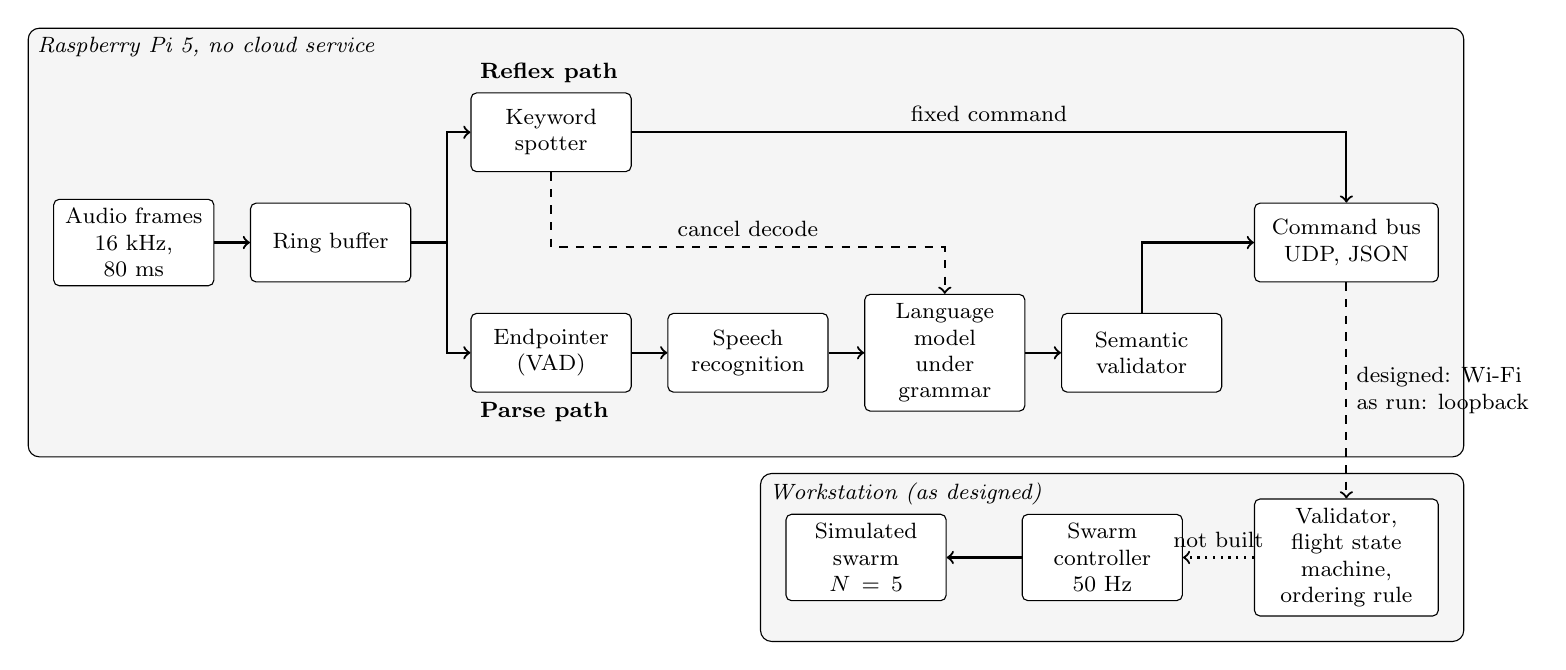
\begin{tikzpicture}[
    font=\footnotesize,
    stage/.style={draw, rounded corners=2pt, align=center, minimum height=10mm,
                  text width=18mm, fill=white},
    flow/.style={->, thick},
    tag/.style={font=\footnotesize\bfseries}]
  \node[stage] (mic) at (0,0)      {Audio frames\\16~kHz, 80~ms};
  \node[stage] (buf) at (2.5,0)    {Ring buffer};
  \node[stage] (kws) at (5.3,1.4)  {Keyword\\spotter};
  \node[stage] (vad) at (5.3,-1.4) {Endpointer\\(VAD)};
  \node[stage] (stt) at (7.8,-1.4) {Speech\\recognition};
  \node[stage] (slm) at (10.3,-1.4) {Language model\\under grammar};
  \node[stage] (val) at (12.8,-1.4) {Semantic\\validator};
  \node[stage, text width=21mm] (bus) at (15.4,0) {Command bus\\UDP, JSON};
  \node[stage, text width=21mm] (fsm) at (15.4,-4.0) {Validator,\\flight state machine,\\ordering rule};
  \node[stage] (ctl) at (12.3,-4.0) {Swarm\\controller\\50~Hz};
  \node[stage] (sim) at (9.3,-4.0)  {Simulated\\swarm\\$N = 5$};
  \draw[flow] (mic) -- (buf);
  \draw[flow] (buf.east) -- ++(0.45,0) |- (kws.west);
  \draw[flow] (buf.east) -- ++(0.45,0) |- (vad.west);
  \draw[flow] (vad) -- (stt);
  \draw[flow] (stt) -- (slm);
  \draw[flow] (slm) -- (val);
  \draw[flow] (kws.east) -| node[pos=0.25, above] {fixed command} (bus.north);
  \draw[flow] (val.north) |- (bus.west);
  \draw[->, thick, dashed] (kws.south) -- ++(0,-0.95) -| node[pos=0.25, above] {cancel decode}
      (slm.north);
  \draw[->, thick, dashed] (bus.south) -- node[right, align=left] {designed: Wi-Fi\\as run: loopback} (fsm.north);
  \draw[->, thick, dotted] (fsm) -- node[above] {not built} (ctl);
  \draw[flow] (ctl) -- (sim);
  \node[tag, anchor=south west] (ta) at (kws.north west) {Reflex path};
  \node[tag, anchor=north west] (tb) at (vad.south west) {Parse path};
  \begin{scope}[on background layer]
    \node[draw, fill=gray!8, rounded corners=4pt, inner sep=9pt,
          fit=(mic) (ta) (tb) (val) (bus),
          label={[font=\footnotesize\itshape, anchor=north west]north west:Raspberry Pi 5, no cloud service}] {};
    \node[draw, fill=gray!8, rounded corners=4pt, inner sep=9pt,
          fit=(sim) (fsm),
          label={[font=\footnotesize\itshape, anchor=north west]north west:Workstation (as designed)}] {};
  \end{scope}
\end{tikzpicture}}
\caption{Dual-path runtime. Both paths read one audio stream and publish to one command bus; the
reflex path publishes a fixed command and cancels any decode in progress. As designed, the bus
carries commands over Wi-Fi to a workstation that runs the state machine, the swarm controller and
the simulation. In the experiments the bus ran over the board's loopback interface, with the consumer
and the state machine on the board, and the link from the state machine to the controller is not
built: formations were commanded to the controller directly (Section~\ref{sec:setup}).}
\label{fig:architecture}
\end{figure*}

The runtime consists of two paths that read the same audio stream and publish to the same command
bus (Fig.~\ref{fig:architecture}). The \emph{parse path} is the general one: a voice-activity
detection (VAD) model (Silero VAD;~\citealp{silero}) segments the stream into utterances, \texttt{whisper.cpp} with the
\texttt{tiny.en} model transcribes each one with an initial prompt that lists the command vocabulary~\citep{whisper,whispercpp}, a fine-tuned Qwen2.5-0.5B
quantised to \QF{}~\citep{qwen25} parses the transcript into a single-line JSON command under a
bounded grammar in the GBNF (GGML Backus--Naur form) formalism served by \texttt{llama.cpp}~\citep{llamacpp}, and a semantic validator checks
the result before it is published. The model, the grammar and the system prompt are taken unchanged
from the companion paper, which selects the model by comparing candidates on accuracy at two quantisation levels and on latency at \QF{} on the same board and reports its exact match of 0.935 on \added[id=PR]{the }reference transcripts\added[id=PR]{ of the 200 golden recordings used here}~\citep{companion}.\chcomment[id=PR]{P2} The
\emph{reflex path} is a two-class keyword spotter that listens continuously and, on detecting
\emph{swarm hold} or \emph{swarm abort}, publishes a fixed command without transcribing anything.

The two paths share no processing stage between the audio buffer and the bus. They are not a fast and a slow
setting of one pipeline: the parse path cannot begin until the endpointer has confirmed the end of
speech, and that wait alone exceeds the reflex budget. The reflex path skips only the stages that
interpret speech; its commands still pass the validator and the state machine. Messages on the bus
are single-line JSON datagrams over the User Datagram Protocol (UDP), each carrying the command, a tag naming the producing path
and a sequence number.

\subsection{Preemption and ordering}
\label{sec:preemption}

When the reflex path fires while the parse path is decoding, two actions follow, and only one is
needed for correctness. The needed one is an ordering rule in the bus consumer: a parse-path message
whose sequence number is lower than that of the latest applied reflex-path message is discarded.
Both paths draw numbers from one locked counter. A parse-path utterance reserves its number when it
is accepted for processing, before transcription, not when its decode completes; a number assigned
at completion would let a slow decode that finishes after a stop compare as newer and override it.
The second action is an optimisation: the reflex path closes the parser's request in flight, so that
the three inference cores are released at once. Correctness does not depend on the cancellation
succeeding; what it governs is recovery, the time before the parse path can accept the next
utterance. The rule covers the utterance in progress, not utterances already queued behind it: a
queued utterance reserves its number when it is dequeued, so after a hold it can still take effect
(after an abort, the state machine rejects it).

\subsection{Reflex-path membership rule}
\label{sec:membership}

\begin{table}
\caption{Reflex-path membership rule applied to the ten intents. A command is admitted only if it
passes both tests; a dash marks a latency test not applied because the fail-safe test has failed.}
\label{tab:membership}
\footnotesize\setlength{\tabcolsep}{3pt}
\begin{tabular*}{\tblwidth}{@{\extracolsep{\fill}}l>{\raggedright\arraybackslash}p{1.75cm}>{\raggedright\arraybackslash}p{2.3cm}l@{}}
\toprule
Intent & Latency-decisive & Fail-safe if false & Path \\
\midrule
\texttt{hover}     & Yes & Yes: stops lateral motion & Reflex \\
\texttt{abort}     & Yes & Yes: descends in place & Reflex \\
\texttt{land}      & No: descent is slow & Yes & Parse \\
\texttt{set\_param} & No & Yes, if it lowers speed & Parse \\
\texttt{unknown}   & No: nothing dispatched & Yes & Parse \\
\AuditDeletedRow{\deleted[id=PR]{\texttt{takeoff}} & \deleted[id=PR]{--} & \deleted[id=PR]{No: spins up rotors} & \deleted[id=PR]{Parse only} \\}
\AuditDeletedRow{\deleted[id=PR]{\texttt{move}} & \deleted[id=PR]{--} & \deleted[id=PR]{No: uncommanded translation} & \deleted[id=PR]{Parse only} \\}
\AuditDeletedRow{\deleted[id=PR]{\texttt{altitude}} & \deleted[id=PR]{--} & \deleted[id=PR]{No: uncommanded climb} & \deleted[id=PR]{Parse only} \\}
\AuditDeletedRow{\deleted[id=PR]{\texttt{rotate}} & \deleted[id=PR]{--} & \deleted[id=PR]{No: uncommanded yaw} & \deleted[id=PR]{Parse only} \\}
\AuditDeletedRow{\deleted[id=PR]{\texttt{formation}} & \deleted[id=PR]{--} & \deleted[id=PR]{No: every vehicle moves} & \deleted[id=PR]{Parse only} \\}
\AuditAddedBlock{\parbox[t]{1.55cm}{\raggedright\texttt{takeoff}, \texttt{move}, \texttt{altitude}, \texttt{rotate}, \texttt{formation}}} & \added[id=PR]{--} & \added[id=PR]{No: each starts or changes motion} & \added[id=PR]{Parse only} \\
\bottomrule
\end{tabular*}
\end{table}

A false trigger on the reflex path publishes a well-formed command that is inside the envelope and
legal in flight, so no validation layer can detect it; the only protection is to restrict which
commands the path carries. A command must pass two tests (Table~\ref{tab:membership}). The first
asks whether the time saved changes the physical outcome. The difference between the parse and
reflex budgets is $2{,}500 - 150 = 2{,}350$~ms; at the validator's speed ceiling of 2.0~m/s that is
4.7~m of travel, comparable to the largest admissible inter-drone spacing (5~m). The second asks what
happens if the command executes without having been spoken: it passes only if the swarm then does
less, never more. Neither test suffices alone. The first alone would admit urgent movements, whose
false triggers are uncommanded motion; the second alone would admit harmless commands that gain
nothing from the fast path but enlarge its false-accept surface.

Exactly two intents pass. \emph{Swarm hold} publishes \texttt{hover}: lateral motion stops and the
mission can be resumed. \emph{Swarm abort} publishes \texttt{abort}, a descent in place with the
motors stopped on ground contact. These are the effects on the designed route; the link that would
apply them to the controller is not built (Section~\ref{sec:setup}), so neither was executed on
the simulated vehicles. A \emph{resume} phrase is excluded deliberately: a false trigger
would restart motion the operator chose to freeze. Confusion between the two admitted classes is
benign, since either outcome stops the swarm. The rule applies to the command a phrase publishes,
not to the phrase, and it states the condition under which a third class could be admitted: both
tests pass, and the aggregate false-accept rate measured with the class in place stays within budget.

\subsection{Validation layers}
\label{sec:layers}

Three layers stand between a decoded command and the vehicles. The \emph{grammar} fixes the form of a
command: every complete decode is a string of the command language, and numbers and drone
identifiers are bounded in length~\citep{companion}. The \emph{semantic validator} enforces the
slots each intent requires and clamps values to a physical envelope rather than rejecting them:
radius 1--10~m, spacing 1--5~m, height 0.5--15~m, speed 0.2--2.0~m/s and distance at most 50~m;
yaw is wrapped into $[-180^\circ, 180^\circ]$. A missing slot or an unparseable or truncated output
resolves to a hold, never to a substituted movement. The \emph{flight state machine} tracks five
states (landed, taking off, flying, landing, aborted) and admits each intent only in the states where
it is legal; a rejected command becomes a hold while airborne and a logged no-op on the ground,
during landing and after an abort. No utterance can leave the aborted state, which only a manual
reset does.

Two error classes pass all three layers by design. An out-of-range value is clamped and executed,
so its motion is bounded but not withheld. And a command that is well-formed, in range and legal,
but not what the operator said, such as a rotation through the right angle in the wrong direction,
passes unchanged, because no layer can compare a command with the speech it came from. A false
trigger on the reflex path belongs to this class. The safe-failure rate measures how often errors
avoid it by resolving to \texttt{unknown} or a hold.

\subsection{Latency budget and core allocation}
\label{sec:budget}

Every stage carries a target at the 95th percentile (p95; p50 and p99 denote the median and the 99th percentile), fixed before any measurement. The end-to-end target of 2,500~ms runs from the moment the endpointer declares the utterance over; the endpointing wait before it is budgeted separately at 500~ms. After that moment, speech recognition is allowed 1,200~ms, language-model prefill 250~ms (assuming a cached prompt prefix), decode 1,100~ms, and validation and dispatch 50~ms. These allowances are ceilings that sum to 2,600~ms, so the end-to-end target is judged on the measured end-to-end figure, not on the sum of stage figures. The reflex path is budgeted at 150~ms from the keyword offset, the end of the
spoken phrase (and 850~ms from its onset, the delay the operator perceives), which isolates what the system adds: the spotter's decision delay, the quantisation of
audio into 80~ms frames, computation and publication. Preemption recovery is budgeted at 300~ms.
The Pi~5's four Cortex-A76 cores are divided between the paths. Core~0 runs the audio frame loop,
which feeds each frame to the keyword spotter and the endpointer and must finish every frame within
its 80~ms period; it never waits for the parse path. Cores 1--3 run speech recognition and the
language model, each with three threads, which never contend because the parser cannot start
before the transcript exists. Pinning separates computation but not memory bandwidth, cache or
temperature, so interference between the paths is measured, not assumed.

\paragraph{Speech components.} The endpointer runs Silero VAD on 32~ms windows; speech starts at a
probability of 0.5 and ends after 450~ms below 0.35, and segments are padded by 200~ms. The keyword
spotter consists of two classifier heads, multilayer perceptrons with two hidden layers of 128 units,
over the frozen feature front end of openWakeWord~\citep{oww}. Each head scores the last 16 speech
embeddings, about 2~s of audio, and a class fires at most once per 1.0~s. The heads were trained on
2,100 synthetic positive clips rendered by three Piper voices~\citep{piper} and 3,930 negative clips
from LibriSpeech~\citep{librispeech}, Speech Commands~\citep{speechcmd} and near-miss clips of
40 authored phrases, weighted five times; the corpora hold 3,000 positive and 5,040 negative clips
(720 of them near misses), the rest being held out for validation and test. One threshold serves
both heads: the highest value on a grid at which both classes keep a validation false-reject rate of
at most 0.05, which selected 0.999. The heads were fitted twice: the first fit was rejected on its
validation results after its test split had been scored once, and the threshold was selected on the
second fit before its test split was scored.

\subsection{Swarm controller}
\label{sec:controller}

The controller returns one acceleration per vehicle every 20~ms (50~Hz) and implements three
formations: a circle, a line and a wedge. Vehicles are assigned to slots once, when the formation is
commanded, by minimising the total squared distance~\citep{turpin2014}. The acceleration sums a
proportional--integral--derivative (PID) law on the slot error ($k_p = 2.0$, $k_i = 0.05$, $k_d = 3.0$, integral limited to $\pm 2.0$), an
artificial potential field that repels pairs closer than 1.5~m~\citep{khatib1986}, and global
flock-centring and velocity-matching terms weighted at 0.15 and 0.25~\citep{reynolds1987}. Because a
force can be outrun at a finite timestep, a geometric clamp after the integrator moves every pair
closer than 0.80~m apart along the line joining them, repeating up to 64 times, and removes their
approaching velocity. A collision is a pair closer than 0.35~m after the clamp. The controller runs
on two simulation backends with the same gains: a kinematic point-mass backend (acceleration at most
4~m/s$^2$, speed at most 3~m/s), on which the clamp can rewrite the state, and a rigid-body PyFlyt
backend~\citep{pyflyt}, which is exercised by smoke tests only and applies no clamp.

\subsection{Experimental setup}
\label{sec:setup}

\paragraph{Platform and thermal state.} All wall-clock measurements were made on a Raspberry Pi~5
with 8~GB of memory, an active cooler, the \texttt{performance} governor and the core allocation of
Section~\ref{sec:budget}. During the latency experiment the processor, sampled at the start of each trial, stayed at 50.5--77.9~$^\circ$C
and the throttle flag was clear on all 360 trials. Audio was replayed from recordings, not captured
from a microphone: in real time through the frame loop in the latency experiment, and faster than
real time in the acoustic-robustness experiment. The bus ran over the loopback interface
with the consumer and state machine on the board.

\paragraph{Latency experiment.} The parse path was timed on the 200 utterances of the golden test
set, recorded by the first author and described in the companion paper~\citep{companion}; the endpointer split them into 226 segments, and each segment is one latency sample. The reflex path was timed on
40 recorded keyword takes by the first author, 20 per class, each replayed twice in two conditions,
80 trials per condition. In the \emph{idle} condition the parse path was resident but idle; in the
\emph{loaded} condition a load thread on cores 1--3 ran the deployed parser back to back on
golden-set transcripts, after 300~s of the same load, so that each trigger met a decode in progress.\added[id=PR]{
Replaying a take reproduces its detection frame (the two passes differ by at most 0.3~ms idle and
12.4~ms loaded), so the second pass is a determinism check, not a second observation: reflex
latencies and counts use the first pass of each take, with exact (Clopper--Pearson) intervals on
counts. Recovery, which waits on the language-model server's once-a-second poll, varies between
passes and uses both. Latency percentiles carry distribution-free 95\% intervals from order
statistics; when the sample cannot bound a p95 from above, only its lower bound is given.}\chcomment[id=PR]{P16, P17}
\added[id=PR]{As a single-path baseline, the 40 takes were also replayed once through the parse path with the
reflex path removed, and each was scored, by the rule of the acoustic-robustness experiment, against
a hold or an abort. The endpointing delay of this baseline, measured from the same offset anchor,
is set by the audio and the endpointer, not by the processor; its later stages were timed on an
x86 workstation, not on the board.}\chcomment[id=PR]{P12: re-time on the Pi}

\paragraph{Keyword-spotter evaluation.} The heads were scored on held-out recordings streamed in
80~ms frames with the runtime's debounce: 300 synthetic test takes per class, 0.429~h of held-out
ambient speech for false accepts, and a stress stream of authored near-miss phrases. False rejects
on the author's voice were scored on the 40 recorded takes. Both keyword criteria are rates
estimated from few events, so each is judged by its 95\% interval (exact binomial for false
rejects, Poisson for false accepts): met if the whole interval lies within the budget, missed if it
lies wholly outside, and otherwise \emph{not demonstrated}.\added[id=PR]{ Detection delay was also measured across
the threshold grid against three estimates of the keyword's end: the exact end sample, known for
575 of the 600 synthetic test takes; and, on the 40 recorded takes, the capture tool's energy bound,
which is the latency experiment's anchor, and the end of the last 32~ms window in which Silero's
speech probability reaches 0.5. This curve was measured after the threshold had been fixed and was
not used to choose it.}\chcomment[id=PR]{P15}

\paragraph{Acoustic-robustness experiment.} The 200 golden recordings were passed through the parse
path once clean and once at each of 20, 15, 10 and 5~dB signal-to-noise ratio, with rotor noise from
the evaluation partition of DREGON~\citep{dregon} mixed against the active speech. The command
recognition rate (CRR) is the fraction of utterances whose dispatched commands all match the
reference \replaced[id=PR]{once both are in canonical form (keys in a fixed order, absent slots omitted, numbers
rounded to one decimal, identifier lists sorted and deduplicated)}{under the canonical comparison of the companion paper}\chcomment[id=PR]{P2}; an utterance split into several
segments counts as recognised only if every command it dispatched is correct. Exact match (EM) on
the reference transcript of the same items gives the parser's own accuracy, so EM minus CRR is the
accuracy the speech stage costs. Word error rate (WER) and the safe-failure rate (the share of failed
utterances resolving to \texttt{unknown} or a hold\added[id=PR]{, with a target of at least 0.70}) are reported per condition. Intervals are 95\%
bootstrap intervals over utterances. Across conditions we report \deleted[id=PR]{a one-way analysis of variance (ANOVA) on the
arcsine-transformed CRR with the Tukey--Kramer comparison~\mbox{\citep{kramer1956}}, }Cochran's
$Q$~\citep{cochran1950}\replaced[id=PR]{ and}{, and} pairwise \added[id=PR]{exact }McNemar tests~\citep{mcnemar1947}\deleted[id=PR]{ (exact below 25 discordant
pairs, continuity-corrected~\mbox{\citep{edwards1948}} from 25 upwards)} at a Bonferroni-corrected~\citep{dunn1961}
$\alpha = 0.0050$\added[id=PR]{; both are paired tests, since every condition reuses the same 200 utterances}.\chcomment[id=PR]{P17} The 200 utterances are paraphrases of 12 command patterns, so intervals and
$p$-values are optimistic. The processor stayed at 54.3--80.1~$^\circ$C; its soft temperature-limit flag was set during the 5~dB condition, which affects timing, not accuracy.

\paragraph{Formation-control experiment.} Formations were commanded to the controller directly,
not spoken, so that control quality is measured apart from recognition. Five vehicles formed a circle
of radius 5~m and a line and a wedge at 2~m spacing, 50 trials each, 60~s per trial on the kinematic
backend. Each trial drew initial positions from a normal distribution with a standard deviation of
0.5~m, seeded by the trial index times 42. Formation accuracy is the fraction of vehicles within
0.5~m of their slot, averaged over the final 5~s; a trial has converged at the first timestep at
which that fraction reaches 0.85. \replaced[id=PR]{Convergence times are summarised by median and interquartile
range. The three formations reuse the same 50 spawns in a deterministic simulator, so no
significance test is reported.}{Convergence times are compared by one-way ANOVA with Tukey's
comparison.}\chcomment[id=PR]{P17}

% =============================================================================
\section{Results}
\label{sec:results}

\subsection{Parse-path latency}
\label{sec:res-parse}

\begin{table}
\caption{Latency budget against measurement on the cooled Raspberry Pi~5 (ms, nearest-rank
percentiles). Parse-path rows count endpointed segments; prefill is the deployed parser's, without a
prompt cache, whereas its target assumes a cached prefix. \replaced[id=PR]{Reflex rows count recorded takes (first
pass; 39 of 40 takes produced a detection in each condition); recovery is measured in the loaded
condition over both passes. 95\% CI: distribution-free interval for the p95 from order statistics;
$\geq$: the sample bounds it from below only. The endpointing wait is a configured constant.}{Reflex rows count detections (78 of 80 trials per condition); recovery is measured in the loaded condition.}\AuditID{P16, P17}}
\label{tab:latency}
\scriptsize\setlength{\tabcolsep}{1.5pt}
\begin{tabular*}{\tblwidth}{@{\extracolsep{\fill}}lrrrrrl@{}}
\toprule
Stage & $n$ & p50 & p95 & \added[id=PR]{95\% CI} & Target & Verdict \\
\midrule
Endpointing wait & 226 & 480 & 480 & \added[id=PR]{--} & 500 & met \\
Speech recognition & 226 & 1,246 & 1,449 & \added[id=PR]{1,418--1,522} & 1,200 & missed \\
Prefill (no cache) & 226 & 570 & 751 & \added[id=PR]{712--791} & 250 & missed \\
Decode & 226 & 561 & 915 & \added[id=PR]{841--950} & 1,100 & met \\
Validation, dispatch & 226 & $<1$ & $<1$ & \added[id=PR]{--} & 50 & met \\
\textbf{End to end, after endpointing} & 226 & 2,441 & 3,122 & \added[id=PR]{3,034--3,305} & 2,500 & missed \\
\midrule
\textbf{Reflex from offset, idle} & \replaced[id=PR]{39}{78} & 195 & 545 & \added[id=PR]{$\geq$436} & 150 & missed \\
\quad spotter delay + frames & \replaced[id=PR]{39}{78} & 190 & 540 & \added[id=PR]{$\geq$430} & -- & \\
\quad Pi compute + publish & \replaced[id=PR]{39}{78} & 5 & \replaced[id=PR]{5}{6} & \added[id=PR]{$\geq$5} & -- & \\
\textbf{Reflex from offset, loaded} & \replaced[id=PR]{39}{78} & \replaced[id=PR]{209}{205} & \replaced[id=PR]{556}{547} & \added[id=PR]{$\geq$436} & 150 & missed \\
\quad spotter delay + frames & \replaced[id=PR]{39}{78} & 190 & 540 & \added[id=PR]{$\geq$430} & -- & \\
\quad Pi compute + publish & \replaced[id=PR]{39}{78} & \replaced[id=PR]{13}{12} & 18 & \added[id=PR]{$\geq$16} & -- & \\
Preemption recovery & 78 & 601 & 1,195 & \added[id=PR]{1,042--1,505} & 300 & missed \\
\bottomrule
\end{tabular*}
\end{table}

\begin{figure}
\centering
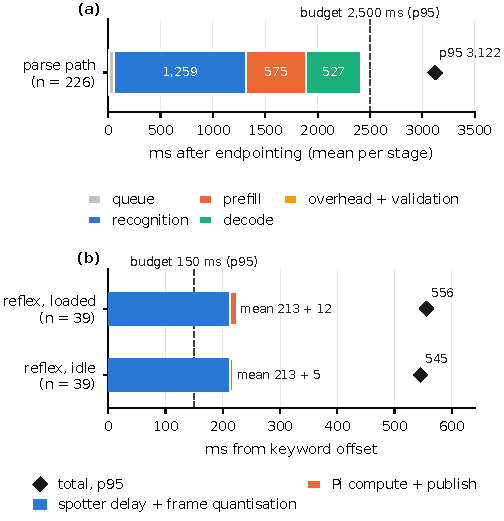
\includegraphics[width=\columnwidth]{figures/fig_latency_paths.pdf}
\caption{Where the time goes on each path. (a) Parse path \replaced[id=PR]{after endpointing}{from the end of speech}: mean time per
stage, stacked (226 segments). (b) Reflex path from the keyword offset, idle and loaded: mean spotter
delay plus frame quantisation, and mean computation and publication on the board (\replaced[id=PR]{first pass of
each of 39 detecting takes}{78 detections
each}).\AuditID{P16, P18} Means add up to the mean total; diamonds mark the measured p95 of the total, since stage
percentiles do not add. Dashed lines: p95 budgets.}
\label{fig:latency}
\end{figure}

The parse path missed its budget (Table~\ref{tab:latency}): its p95 from the endpointer's end-of-utterance decision was
3,122~ms over 226 segments, 622~ms (25\%) above 2,500~ms, and 3,602~ms with the endpointing wait
included. Two stages missed their allowances: speech recognition at 1,449~ms against 1,200~ms, and
prefill at 751~ms against 250~ms, measured without a prompt cache. Decode met its allowance at
915~ms, as did the endpointing wait (480~ms) and validation with dispatch (under 1~ms). Prefill and
decode together took 1,658~ms at p95, against the 1,350~ms sum of their allowances, and the shortest
speech-recognition time of any segment was 1,063~ms. Two intervals without a budget row, the wait for the parse-path worker and
the overhead of the requests to the language-model server, were 73~ms and 8~ms at p95.
Fig.~\ref{fig:latency}a shows speech recognition as the largest share of the mean.\added[id=PR]{ Every verdict
in Table~\ref{tab:latency} that has an interval holds over the whole interval of its p95: the end-to-end interval,
3,034--3,305~ms, lies above 2,500~ms, and the decode interval, 841--950~ms, below 1,100~ms.}\chcomment[id=PR]{P17}

\subsection{Reflex path and preemption}
\label{sec:res-reflex}

The reflex path missed its 150~ms budget in both conditions, at 545~ms idle and \replaced[id=PR]{556}{547}~ms loaded
(p95\added[id=PR]{ over 39 takes; the 95\% lower bound, 436~ms, already exceeds the budget}). The spotter's decision delay and the frame quantisation accounted for 540~ms at p95 in both
conditions, and the board's computation and publication for \replaced[id=PR]{5}{6}~ms idle and 18~ms loaded
(Table~\ref{tab:latency}; Fig.~\ref{fig:latency}b). The offset anchor is an energy-based estimate,
and on \replaced[id=PR]{3 of 39 idle and 2 of 39 loaded}{6 of 78 idle and 4 of 78 loaded} takes the command was published before it, by up to 235~ms.\chcomment[id=PR]{P16}
Under load no frame exceeded the 80~ms period: the frame loop's computation was 14.2~ms at the
median, 22.9~ms at p99 and 45.5~ms at most. While speech recognition ran, the longest frame took 74.2~ms. From the keyword onset the reflex path took 1,265~ms idle
and 1,266~ms loaded at p95, against an 850~ms target.

\replaced[id=PR]{Under load, 39 of the 40 takes produced a detection, and each of the 39 found a parse-path decode in
progress and cancelled it (39 of 39; 95\% interval of the cancellation rate 0.910--1.000)}{Of the 80 loaded trials, 78 produced a detection, and each of the 78 found a parse-path decode in
progress and cancelled it}; no cancelled decode completed, so the ordering rule was never exercised
by a trial and is verified by the consumer's unit tests. In both conditions all \replaced[id=PR]{20 abort takes}{40 abort trials} fired
the abort class and \replaced[id=PR]{19 of 20 hold takes}{38 of 40 hold trials} fired the hold class, the \replaced[id=PR]{miss being the same take on both}{two misses being one take on both}
replays; no take fired the other class\added[id=PR]{ (0 of 40; 95\% upper bound 0.088)}.\chcomment[id=PR]{P16} While listening to the 200 golden utterances, the reflex path
fired once, a \texttt{hover} during a landing command; the offline scoring of the same recordings
(Section~\ref{sec:res-kws}) produced no false accept, and the records do not explain the difference.
Preemption recovery, measured until the language-model server reported its slot idle, missed its
budget at 1,195~ms (p95; median 601~ms; maximum 1,505~ms) against 300~ms. The cancelled request itself returned within 6.5~ms of the trigger at p95.

\subsection{\added[id=PR]{Single-path baseline}}
\label{sec:res-single}

\added[id=PR]{Replayed through the parse path alone, 37 of the 40 stop takes were recognised (miss rate 0.075,
95\% interval 0.016--0.204). The recogniser transcribed two abort takes as ``swarma boards'' and one
hold take as ``swarm, walled'', and the parser turned all three into a formation command; none
resolved to a hold. The reflex path had stopped all three with the right class, and the one take it
missed, a hold, was recognised by the parse path. Before the parse path could start, the endpointer
declared each utterance over 612~ms after the keyword offset at the median (95\% interval 600--652~ms)
and 742~ms at p95: the wait alone exceeds the reflex path's whole p95 of 545~ms from the same anchor.
On the workstation, the single path took 2,271~ms from the keyword offset to the applied command at
the median and 2,768~ms at p95. On the board, the parse path's stages after endpointing were measured
only on the ten golden utterances whose command is a bare hold or abort, at a median of 1,902~ms;
adding the shortest endpointing delay observed here (320~ms) to the shortest of those (1,748~ms) gives
an estimate of 2.1~s, not a measurement, for a stop routed through the parse path on the board.}

\added[id=PR]{Read together, the two runs show a case that the ordering rule does not cover. On each of the 39
takes the reflex path detected, its message was published before the endpointer had accepted the
utterance, so the parse of the stop phrase itself reserves a later sequence number and is applied
after the stop. Parsed correctly, it repeats the stop. On the hold take that became a formation
command, it would have replaced the hold with a formation change about two seconds later; after the
two aborts, the state machine would have rejected it. This combined behaviour is inferred, not
measured: the latency experiment did not pass the keyword takes to the parse path.}\chcomment[id=PR]{P12}

\subsection{Keyword spotter}
\label{sec:res-kws}

\begin{figure}
\centering
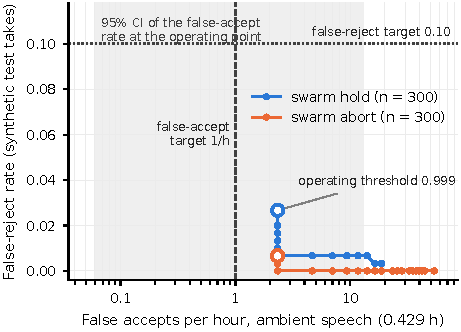
\includegraphics[width=\columnwidth]{figures/fig_keyword_curve.pdf}
\caption{Keyword-spotter operating curve on the held-out test split: false-reject rate on 300
synthetic takes per class against false accepts per hour on 0.429~h of ambient speech (both classes
together), as the common threshold sweeps the selection grid. Open circles: operating threshold
0.999; shaded band: 95\% Poisson interval of its false-accept rate; dashed and dotted lines: targets. The false-reject criterion is judged on the author's recorded takes (Section~\ref{sec:res-kws}), not on these synthetic takes.}
\label{fig:kws}
\end{figure}

At the operating threshold of 0.999 (Fig.~\ref{fig:kws}), the ambient-speech test stream produced
one false accept in 0.429~h, 2.33 per hour with a 95\% interval of [0.06, 12.98], against a target of
at most one per hour; the criterion is not demonstrated. The validation stream (0.167~h) and the
golden-set recordings (0.304~h) produced none. A stress stream of authored near-miss phrases produced
34 false accepts in 0.100~h, 31 of them on the hold head; it is a stress condition, not an operating rate, and no criterion is judged on it. On the synthetic test takes, rendered by the three voices used in training, the
false-reject rate was 0.027 for hold and 0.007 for abort; on the author's 40 recorded takes it was
0.050 [0.001, 0.249] for hold and 0.000 [0.000, 0.168] for abort, against a target of at most 0.10,
so this criterion is not demonstrated either.\deleted[id=PR]{ Measured from the synthetic takes' own anchor, the
spotter's delay was 131--188~ms at p95.} The curve is flat in false accepts above a threshold of
0.88: the single test false accept survives every threshold in that range.

\AuditAddedBlock{%
\begin{table}
\caption{Keyword-spotter delay against the common threshold (ms, nearest-rank p95 unless marked).
Exact: from the known end sample of 575 synthetic test takes. Energy and Silero: from two estimates
of the keyword's end on the 40 recorded takes; energy is the anchor of Table~\ref{tab:latency}. False
accepts per hour on the author's 0.304~h of golden-set recordings and on the 0.429~h ambient
stream. Bold: operating threshold.\AuditID{P15}}
\label{tab:delay}
\footnotesize\setlength{\tabcolsep}{3pt}
\begin{tabular*}{\tblwidth}{@{\extracolsep{\fill}}lrrrrrr@{}}
\toprule
& Exact & \multicolumn{2}{c}{Energy} & Silero & \multicolumn{2}{c}{False accepts/h} \\
\cmidrule(lr){3-4}\cmidrule(lr){6-7}
Threshold & p95 & p50 & p95 & p95 & Golden & Ambient \\
\midrule
0.5   &  85 &  80 & 230 & 152 & 42.8 & 16.3 \\
0.9   &  94 & 140 & 230 & 152 & 26.3 &  2.3 \\
0.98  & 110 & 150 & 260 & 168 & 13.2 &  2.3 \\
0.99  & 113 & 160 & 470 & 392 & 13.2 &  2.3 \\
\textbf{0.999} & 152 & 190 & 540 & 424 &  0.0 &  2.3 \\
\bottomrule
\end{tabular*}
\end{table}}

\added[id=PR]{Table~\ref{tab:delay} gives the spotter's delay across the threshold grid. From the exact end
sample, the p95 at the operating threshold was 152~ms (95\% interval 131--216~ms; hold 179~ms, abort
131~ms), and 110~ms at 0.98. On the recorded takes, from the energy anchor, it was 540~ms at the
operating threshold, 260~ms at 0.98 and 230~ms from 0.9 downwards; no threshold in the grid brought it
within 150~ms, and the lower bound of its interval was at least 200~ms at every threshold. The two
estimates of a recorded keyword's end disagreed by more than the budget: Silero's end came a median
116~ms after the energy bound (range $-184$ to $+296$~ms), and measured from it the p95 at the
operating threshold was 424~ms. Lower thresholds traded delay for false accepts on the operator's own
speech: the golden-set recordings produced none at 0.999, one at 0.998, four at 0.98 and eight at
0.9. The false-reject rate on the recorded takes was 0.025 (1 of 40) from 0.998 upwards and zero
below.}\chcomment[id=PR]{P15}

\subsection{Acoustic robustness}
\label{sec:res-acoustic}

\begin{table*}[t]
\caption{Acoustic robustness of the parse path on the 200 golden recordings under rotor noise, on
the Raspberry Pi~5. EM on the reference transcripts is 0.935 in every condition, so EM $-$ CRR is the
accuracy lost in the speech stage. Brackets: 95\% bootstrap intervals over utterances.}
\label{tab:acoustic}
\footnotesize
\begin{tabular*}{\textwidth}{@{\extracolsep{\fill}}lcccc@{}}
\toprule
Condition & CRR & WER (\%) & EM $-$ CRR & Safe-failure rate \\
\midrule
Clean & 0.690 [0.625, 0.750] & 23.3 [20.2, 26.6] & 0.245 [0.185, 0.310] & 0.032 (2 of 62) \\
20 dB & 0.675 [0.610, 0.740] & 24.3 [21.6, 27.2] & 0.260 [0.200, 0.325] & 0.015 (1 of 65) \\
15 dB & 0.650 [0.585, 0.715] & 26.1 [23.4, 29.1] & 0.285 [0.225, 0.350] & 0.014 (1 of 70) \\
10 dB & 0.590 [0.520, 0.660] & 28.8 [25.9, 31.7] & 0.345 [0.280, 0.410] & 0.024 (2 of 82) \\
5 dB  & 0.485 [0.415, 0.555] & 36.0 [32.9, 39.3] & 0.450 [0.380, 0.520] & 0.039 (4 of 103) \\
\bottomrule
\end{tabular*}
\end{table*}

\AuditDeletedBlock{%
\begin{figure}
\centering
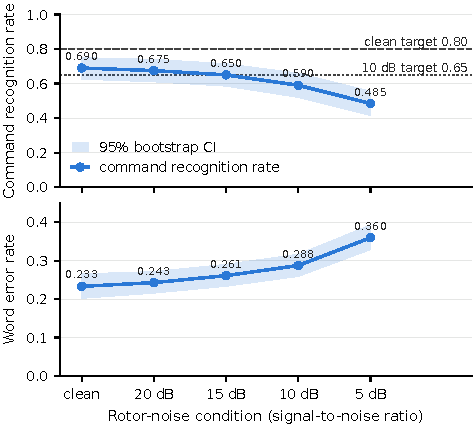
\includegraphics[width=\columnwidth]{figures/fig_snr.pdf}
\caption{Command recognition rate (top) and word error rate (bottom) against rotor-noise level on
the 200 golden recordings, with 95\% bootstrap intervals. Dashed and dotted lines: the clean-audio
target of 0.80 and the 10~dB target of 0.65.}
\label{fig:snr}
\end{figure}}\AuditID{P18}

In clean audio the CRR was 0.690 [0.625, 0.750] against a target of at least 0.80
(Table~\ref{tab:acoustic}); the parser alone reached an EM of 0.935 on the same items, so the speech
stage cost 0.245. Each of the 62 clean failures was assigned one cause in a fixed order: endpointer
splits accounted for 22 (23 of the 200 utterances, 11.5\%, were split at a pause and all 23 failed; one is counted under the parser-error cause, which is assigned first),
recognition errors that left the intent right but a slot wrong for 23, recognition errors that changed
the intent for 5, and parser errors already present on the reference text for 12. Scored on the last
segment of each utterance only, the clean CRR was 0.730. At 10~dB the CRR was 0.590 [0.520, 0.660]
against a target of at least 0.65 (\replaced[id=PR]{Table~\ref{tab:acoustic}}{Fig.~\mbox{\ref{fig:snr}}}); recognition errors that changed the intent
rose from 5 to 19 and those that corrupted a slot from 23 to 30, while parser errors stayed at 12.
The CRR reached 0.80 at no level and held at 0.65 or above down to 15~dB on the point estimate.

\deleted[id=PR]{The ANOVA rejected equality across the five conditions ($F(4, 995) = 6.03$, $p = 8.6 \times
10^{-5}$), and Tukey's comparison separated 5~dB from clean, 20 and 15~dB. The five conditions reuse the same 200 utterances, so the paired tests below are the primary analysis. }Cochran's $Q$ \deleted[id=PR]{also }
rejected equality \added[id=PR]{across the five conditions }($Q = 61.05$, 4 degrees of freedom, $p = 1.7 \times 10^{-12}$), and the pairwise
\added[id=PR]{exact }McNemar tests separated \replaced[id=PR]{clean audio and 20~dB from 10 and 5~dB, and 15 and 10~dB from
5~dB; two of these pairs, 20 against 10~dB and 10 against 5~dB, pass the corrected threshold
narrowly ($p = 0.0046$ each)}{clean audio from 10 and 5~dB, and 20 and 15~dB from 5~dB}.\chcomment[id=PR]{P17} The safe-failure
rate lay between 0.014 and 0.039 at every level, against a target of at least 0.70: failures grew
from 62 to 103 while safe failures stayed between one and four. On the reference transcripts the
parser made 13 failures (an EM of 0.935~\citep{companion}), none of them safe. Speech recognition differed between the board and the
workstation on two to six transcripts per condition, which moved the 5~dB CRR from 0.495 on the
workstation to 0.485 on the board; the board's figures are reported.

\subsection{Formation control}
\label{sec:res-formation}

\AuditDeletedBlock{%
\begin{figure*}[t]
\centering
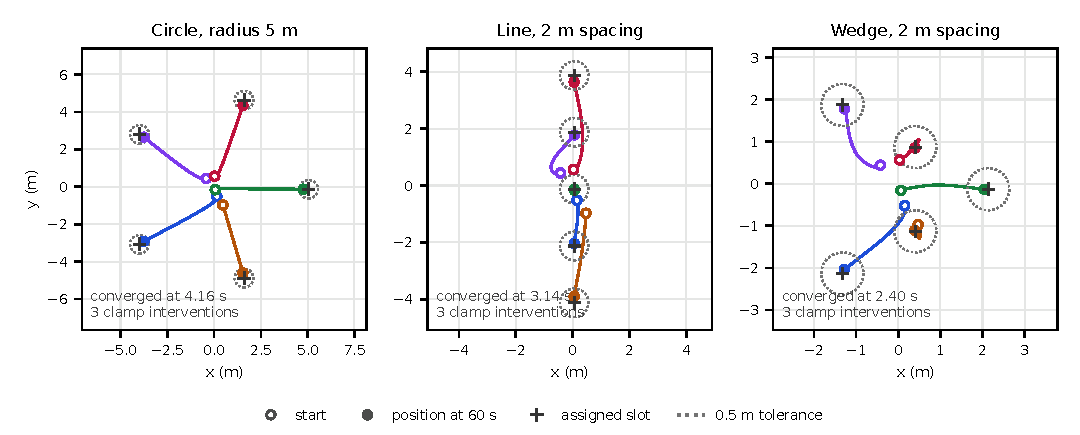
\includegraphics[width=0.85\textwidth]{figures/fig_trajectories.pdf}
\caption{Trajectories of the five simulated vehicles in one trial of each formation on the kinematic
backend: start (open circle), position at 60~s (filled circle), assigned slot (cross) and the 0.5~m
formation-accuracy tolerance (dotted circle). Trial 1 (seed 42) of each formation; colours identify vehicles.}
\label{fig:trajectories}
\end{figure*}}\AuditID{P18}

\begin{figure}
\centering
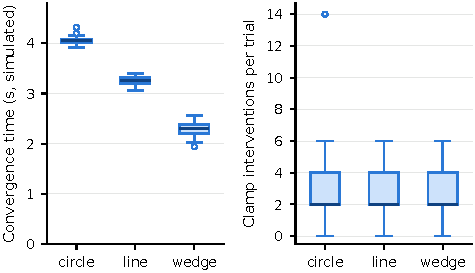
\includegraphics[width=\columnwidth]{figures/fig_formation_boxes.pdf}
\caption{Convergence time (left, simulated seconds) and separation-clamp interventions per trial
(right) over 50 trials of each formation on the kinematic backend. Boxes: interquartile range; line: median; whiskers: 1.5 times the interquartile range; circles: outliers.}
\label{fig:boxes}
\end{figure}

All 150 trials converged\deleted[id=PR]{ (Fig.~\mbox{\ref{fig:trajectories}} shows one trial of each formation)}, the slowest after 4.32~s, and formation
accuracy was 1.000 in every trial. Median convergence time was 4.06~s for the circle (interquartile
range 4.00--4.08~s), 3.26~s for the line (3.21--3.32~s) and 2.30~s for the wedge (2.21--2.38~s)
(Fig.~\ref{fig:boxes})\replaced[id=PR]{; the interquartile ranges do not overlap}{. The ANOVA rejected equality ($F(2, 147) = 3500.7$,
$p = 1.0 \times 10^{-124}$), and Tukey's comparison separated every pair: the circle took 0.795~s
longer than the line (95\% interval [0.745, 0.845]) and 1.755~s longer than the wedge ([1.705, 1.805]),
and the line 0.960~s longer than the wedge ([0.910, 1.010])}.\chcomment[id=PR]{P17} At the end of each trial, the mean
distance of a vehicle from its slot was 0.29~m for the circle, 0.13~m for the line and 0.07~m for the
wedge. No collision was observed in any trial\added[id=PR]{, as the clamp guarantees}. The separation clamp intervened 432 times (150 in
the circle trials, 141 in the line and 141 in the wedge), between 0 and 14 times per trial, and
intervened in 144 of the 150 trials. \replaced[id=PR]{Of the 432 interventions, 423 came on the first tick of a trial,
before the controller had moved any vehicle: 48 of the 50 spawns, which the three formations
share, place at least one pair closer than 0.80~m (141 pairs in all), and the clamp separates them.
The other 9 occurred in flight, all in one circle trial. The closest approach of 0.800~m in those
144 trials is therefore the clamp's correction of the initial placement; in the six trials whose
spawn held no close pair, the vehicles stayed 0.82--0.89~m apart without the clamp acting.}{The closest approach was 0.800~m, the clamp distance, in each
of those 144 trials, and 0.82--0.89~m in the other six.}\chcomment[id=PR]{P14}

\subsection{Summary against the requirements}
\label{sec:res-summary}

\begin{table}
\caption{Every requirement of the system\deleted[id=PR]{ other than the safe-failure target, which is defined in
the companion paper and reported in Section~\mbox{\ref{sec:res-acoustic}}}, with its measured result.\added[id=PR]{ Engineering checks
(simulation backends, state-machine legality, per-stage attribution) are reported in the text.} ``Not dem.'' (not demonstrated): the 95\%
interval straddles the target. ``Not run'': requires an end-to-end run with networking disabled,
which was not performed.\added[id=PR]{ ``By constr.'': holds by construction, so the trial count is not evidence.}\AuditID{P14, P16}}
\label{tab:summary}
\footnotesize\setlength{\tabcolsep}{2.5pt}
\begin{tabular*}{\tblwidth}{@{\extracolsep{\fill}}>{\raggedright\arraybackslash}p{2.9cm}>{\raggedright\arraybackslash}p{3.1cm}l@{}}
\toprule
Requirement & Measured & Verdict \\
\midrule
Reflex path preempts the parse path & \replaced[id=PR]{39/39 takes cancelled the decode}{78/78 decodes cancelled}; 0 cross-triggers & met \\
Formation control, five drones & 150/150 trials converged & met \\
\AuditDeletedRow{\deleted[id=PR]{Two simulation backends} & \deleted[id=PR]{Smoke tests pass, same gains} & \deleted[id=PR]{met} \\}
\AuditDeletedRow{\deleted[id=PR]{Flight state machine} & \deleted[id=PR]{Every legality case tested} & \deleted[id=PR]{met} \\}
\AuditDeletedRow{\deleted[id=PR]{Per-stage attribution} & \deleted[id=PR]{All five stages, p50 and p95} & \deleted[id=PR]{met} \\}
Collisions & 0 in 150 trials (clamp) & \replaced[id=PR]{by constr.}{met} \\
Formation accuracy $\geq 0.85$ & 1.000 in every trial & met \\
Reflex latency $\leq 150$~ms & 545 idle, \replaced[id=PR]{556}{547} loaded & missed \\
End to end $\leq 2{,}500$~ms & 3,122 & missed \\
Recovery $\leq 300$~ms & 1,195 & missed \\
Clean CRR $\geq 0.80$ & 0.690 & missed \\
CRR at 10~dB $\geq 0.65$ & 0.590 & missed \\
\added[id=PR]{Safe-failure rate $\geq 0.70$} & \added[id=PR]{0.014--0.039} & \added[id=PR]{missed} \\
Keyword false accepts $\leq 1$/h & 2.33 [0.06, 12.98] & not dem. \\
Keyword false rejects $\leq 0.10$ & hold 0.050 [0.001, 0.249], abort 0.000 [0.000, 0.168] & not dem. \\
Offline speech recognition & -- & not run \\
Offline operation & -- & not run \\
Live demonstration & -- & not performed \\
\bottomrule
\end{tabular*}
\end{table}

Table~\ref{tab:summary} collects the \replaced[id=PR]{fifteen requirements: three are met, one holds by construction, six are
missed, two are not demonstrated, two have not been run, and the live demonstration was not
performed. Three engineering checks also pass: both simulation backends run with the same gains,
the flight state machine passes a test of every legality case, and every stage of both paths is
attributed at p50 and p95.}{seventeen requirements: six are met, one holds by construction, five are missed, two
are not demonstrated, two have not been run, and the live demonstration was not performed. The
safe-failure target, defined in the companion paper, is also missed at every noise level.}\chcomment[id=PR]{P2, P18}

% =============================================================================
\section{Discussion}
\label{sec:discussion}

\paragraph{The reflex path: design held, budget missed.} The behaviour the dual-path design exists
for was observed without exception: every trigger that met a decode cancelled it, the two classes
were never confused on the recorded takes, and loading the language model added \replaced[id=PR]{13}{12}~ms at p95 to the board's share of the
reflex latency without delaying any audio frame. The 150~ms budget was nevertheless missed by a wide margin,
and the measurement locates the miss in the 540~ms before publication that the spotter's decision
delay, the 80~ms frame quantisation and the imprecision of the offset anchor share, not in the
board's \replaced[id=PR]{5--18}{6--18}~ms.\chcomment[id=PR]{P16} The core allocation therefore did what it was designed to do, and reducing the
reflex latency requires changing the spotter, not the board. \replaced[id=PR]{The delay--threshold curve
(Table~\ref{tab:delay}) splits the 540~ms further. Measured from an exact anchor, the spotter's own
p95 is 152~ms, about the budget; on the recorded takes most of the excess appears only above a
threshold of 0.98, where the heads' scores saturate, and the two estimates of where a recorded
keyword ends differ by up to 300~ms, twice the budget. Lowering the threshold would shorten the
delay but raise false accepts on the operator's own commands, and it would not reach 150~ms at p95
on the energy anchor at any threshold tested. A new operating point would therefore have to be
chosen on validation data and re-measured on new takes against an anchor more precise than either
estimate, such as a forced alignment.}{The spotter's delay on the synthetic
takes (131--188~ms at p95) was measured from a different anchor, so the two figures are not directly
comparable.}\chcomment[id=PR]{P15} Recovery after preemption is limited mainly by the
language-model server, which registers a closed connection by polling once per second; its p95 and
maximum exceed that period, so the polling explains only part of it, and an explicit slot
cancellation is the first change to measure. \replaced[id=PR]{On the same 40 takes and the same anchor, the
parse path alone could not start before 612~ms of endpointing at the median, longer than the reflex
path's p95, and it turned 3 of the 40 stops into a formation command (Section~\ref{sec:res-single}).
The case for a separate path therefore rests on robustness as much as on speed, and the endpointing
part of it does not depend on the board. The same comparison exposes a gap in the ordering rule: the
parse of the stop phrase itself is accepted after the reflex message and can replace a hold.
Reserving the parse-path number at the onset of speech rather than at acceptance would make that
parse stale, at the cost of also discarding a command spoken in the same utterance as the stop.}{For comparison with the parse path, its p95 from the
true end of speech, including the endpointing wait, was 3,602~ms, against 545~ms for the reflex path
from the keyword offset.}\chcomment[id=PR]{P12}

\paragraph{The parse path.} Two stages explain the 622~ms excess. Prefill without a prompt cache
cost 751~ms against a 250~ms allowance; the deployed parser disables the cache so that its accuracy
is exactly the one measured in the companion paper, whose timing with a cached prefix gave a prefill
p95 of 328.8~ms on the same board~\citep{companion}. Whether caching changes the decoded commands was
not tested, so enabling it requires a parity check. Speech recognition exceeded its allowance by
249~ms; an optimised acoustic model or a streaming encoder could reduce it, at a possible cost in
accuracy; such a change would have to be selected on a held-out recording set rather than on the golden set,
which is the test set.

\paragraph{Errors do not become safer under noise.} Noise added failures, and nearly all of the
added failures dispatched an executable command rather than a hold. The same tendency appears on
reference text, where the parser declines almost never on in-domain input~\citep{companion}. The
validation layers cannot compensate: a misrecognised slot within the envelope, or a wrong but legal
intent, passes all three. The membership rule, which keeps such errors off the reflex path, and the
state machine, which keeps them from undoing an abort, bound the damage; they do not prevent it. A
confidence gate that routes low-probability decodes to \texttt{unknown} is the next measurement.\added[id=PR]{
The parse path also acts on speech that is not a command. On the companion paper's
out-of-domain set, the deployed parser dispatched an executable command for 38 of 150 inputs
(0.253, against a target of at most 0.05)~\citep{companion}. With no wake word, push-to-talk or
confirmation in front of it, the parse path exposes the swarm to bystander speech, a larger
false-command exposure than the reflex path's false accepts, which the membership rule
restricts to a hold or an abort.}\chcomment[id=PR]{P16}
The endpointer's splits are a separate cost: scoring only the last segment would have raised the
clean CRR to 0.730, still below the 0.80 target, and a change of scoring rule is not a change to the
system.

\paragraph{\replaced[id=PR]{What the collision result shows.}{The separation clamp carries the collision result.}} \replaced[id=PR]{Zero collisions in 150 trials holds by
construction: a collision is counted after the clamp, which leaves no pair closer than 0.80~m. The
clamp's interventions are not evidence against the potential field either. Almost all of them
separated vehicles that spawned too close, before the controller acted; only 9, all in one circle
trial, came in flight, and in the six trials whose spawn held no close pair the field kept the
vehicles apart unaided. Whether the field alone avoids collisions in general was not tested; a run without the clamp
would test it.}{Zero collisions in 150 trials
follows from the clamp, not from the potential field: the field alone let pairs inside 0.80~m 432
times, in 144 of 150 trials, and in every trial in which the clamp intervened the closest approach
equals the clamp distance.}\chcomment[id=PR]{P14} A real
airframe exposes no state to rewrite, so on hardware the same mechanism would have to act through
commanded accelerations or thrust. Formation accuracy is saturated by the protocol and does not
discriminate between the formations; convergence time does.

\paragraph{Comparison by design.} The nearest local baseline, the agent of \citet{lim2025}, prompts
open models of the same families on a workstation GPU, accepts typed text, flies one vehicle,
relies on a human to switch to position mode as its fallback, and reports no latency. Our system takes
speech on a CPU-only board, fine-tunes and constrains its model, commands five vehicles, and carries
its stop in software under a measured budget. The two are therefore compared by design rather than by
measurement. CommandSwarm~\citep{commandswarm2026} shares our use of deterministic gates, and
SkySim~\citep{skysim2026} our hold on rejection; neither reports running on a single-board computer,
and neither separates its stop from the interpreting path. MIRA's gate aborts at a median of 466~ms from speech onset~\citep{mira}; our reflex path took 965~ms at the median from keyword onset. What it adds over that gate is therefore not speed but a trigger restricted to two commands by a derived rule, and a budget against which its latency is located.

\paragraph{Limitations.} The formation results come from a kinematic simulator without rotor
dynamics, wind or downwash; the rigid-body backend was exercised by smoke tests only, at an effective
control rate of 24~Hz, and no physical flight was performed. The audio was replayed recordings of one
speaker in one session, not live capture. The bus ran over loopback, so no wireless hop and no loss
of its unacknowledged UDP datagrams was measured. The link from the state machine to the controller is
not built, and formations were commanded directly; no run joined speech to formation, and the
effects of a hold or an abort on the vehicles, including the time to rest, were not measured. Offline
operation was not verified by a run with networking disabled, and the live demonstration was not
performed. Formation commands carry no speed, so the validator's 2.0~m/s ceiling does not apply to
formation changes, while the backends allow 3~m/s; vehicle speeds were not recorded. Preemption does
not reach utterances queued behind the one in progress, nor a trigger that arrives during
transcription, and no reflex trial overlapped speech recognition.\added[id=PR]{ The single-path baseline's stages
after endpointing were timed on a workstation, and the interaction between a reflex stop and the
parse of the same phrase was inferred from two separate runs rather than measured.}\chcomment[id=PR]{P12} The state machine judges legality on a command's intent before the validator substitutes a hold, so an unvalidated command could dispatch a hold in a state where a hold is illegal; on the deployed route validation comes first, so the case does not arise there. Finally, the 20 recorded takes per class and the 0.429~h ambient stream are too small
to decide either keyword criterion.

% =============================================================================
\section{Conclusion}
\label{sec:conclusion}

A dual-path voice interface for a swarm of five simulated drones can run its speech and language
stages on a Raspberry Pi~5, on recorded audio, with a fine-tuned small language model, and a
keyword-spotter reflex path can preempt that model: every trigger during inference cancelled the
decode, and the board added only \replaced[id=PR]{5--18}{6--18}~ms before the stop was published on the bus, although neither keyword-spotter error
criterion is demonstrated and recovery after preemption missed its budget.
A two-test membership rule restricts the reflex path to a hold and an abort, and three validation
layers bound what a wrong command can do. The system misses its latency budgets on both paths, before the board's share on the reflex path
and in speech recognition and uncached prefill on the parse path, and misses its recognition targets under
rotor noise, with errors that do not become safer as noise rises.\added[id=PR]{ Routed through the parse path
alone, a stop waited 612~ms at the median for the endpointer and was misrecognised in 3 of 40 takes.}\chcomment[id=PR]{P12}
Future work will reduce the spotter's
decision delay\added[id=PR]{ and re-measure it against a forced alignment, reserve the parse-path sequence
number at the onset of speech}, cache the prompt prefix after a parity check, replace the server's polling with an
explicit slot cancellation, flush queued utterances on a trigger, add a confidence gate, build the
link from the state machine to the controller, replace the integrator clamp with a force-level
mechanism, and run the complete chain live, with networking disabled and on physical vehicles.

% =============================================================================
\printcredits

\section*{Funding}
This research did not receive any specific grant from funding agencies in the public, commercial,
or not-for-profit sectors.

\section*{Declaration of competing interest}
The authors declare that they have no known competing financial interests or personal
relationships that could have appeared to influence the work reported in this paper.

\section*{Data availability}
The runtime, the swarm controller and simulation backends, the keyword-spotter training and
evaluation scripts, the golden-set and keyword recordings, the raw records of every experiment and
the scripts that produce every table and figure in this article\deleted[id=PR]{ except Fig.~\mbox{\ref{fig:trajectories}}, which is distributed as rendered}, are publicly available at
\url{https://github.com/TayebKahia/voice-swarm-edge-}. The deployed language-model artefact is
distributed through the repository's releases.\added[id=PR]{ Code is released under the MIT licence and the authors' data, recordings and results under
CC~BY~4.0. The recordings are of the first author, who consents to their release. Third-party
corpora (DREGON, LibriSpeech, Speech Commands) are not redistributed; the published scripts
regenerate the noise-mixed audio and the keyword-spotter negatives from them under their own licences, and model
weights keep the licences of their base models.}\chcomment[id=PR]{P1}

\section*{Declaration of generative AI and AI-assisted technologies in the writing process}
\replaced[id=PR]{During the preparation of this work the authors used Claude (Anthropic) for drafting and language editing. After using this tool, the authors reviewed and edited the content as needed and take full responsibility for the content of the publication.}{During the preparation of this work the authors used Claude (Anthropic) in order to assist with the writing of the manuscript.
The authors reviewed the content and take full responsibility for the publication.}\chcomment[id=PR]{Minor 17}

\bibliographystyle{cas-model2-names}
\bibliography{references}

\end{document}
